\documentclass{article}
\usepackage[utf8]{inputenc}
\usepackage[margin=1in]{geometry}
\usepackage{xcolor, tikz, amsmath, amsthm, fancyhdr, xfrac, physics, cleveref}

\pagecolor[rgb]{0.2,0.2,0.2}
\color[rgb]{1,1,1}

% Headers
\pagestyle{fancy}
\fancyhf{}
\rhead{Max Ortner}
\lhead{Calculus III}
\chead{Problem Set \#1}
\cfoot{Page \thepage}
\renewcommand{\headrulewidth}{0pt}
\renewcommand{\footrulewidth}{0pt}

\newcommand{\nhat}[1]{\boldsymbol{\hat{\textbf{#1}}}}

\newcommand{\qnumber}[1]{
\vspace{0.5cm}
\noindent
\textbf{#1.}
\vspace{4mm}
}

\setlength{\parskip}{0.15cm}
%\setlength{\parindent}{0em}
\renewcommand{\baselinestretch}{1.2}

\newtheorem{theorem}{Theorem}

\begin{document}


\qnumber{5}

\begin{figure}[h]
    \centering

    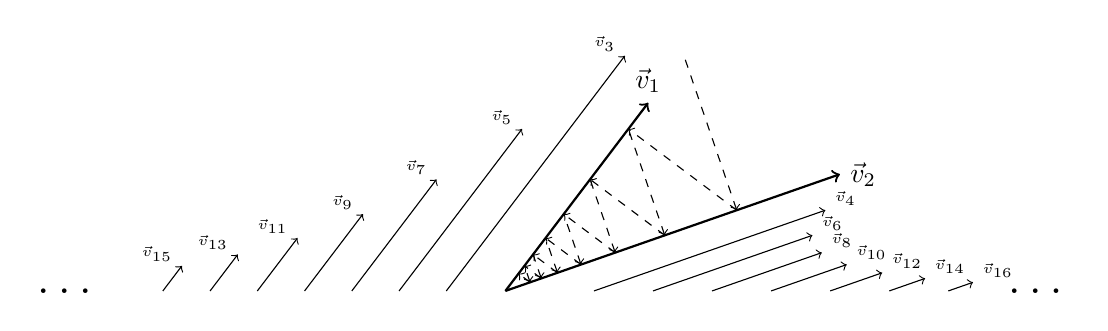
\begin{tikzpicture}[scale=1.5]
        \draw[->, thick] (0, 0) -- ( 0.9442 * 3.0, 0.32942 * 3.0) node[right] {$\vec{v}_2$};
        \draw[->, thick] (0, 0) -- (0.60473 * 2.0, 0.79643 * 2.0) node[left, above]  {$\vec{v}_1$};

        % Unit vector v_2
        \foreach \i in {1, 3, 5, 7, ..., 13} {
            \pgfmathsetmacro\result{\i + 3}
            \draw[->] (\i/4 + 1/2, 0) -- ( 0.9442 * 2.5 * 0.83^\i + \i/4 + 1/2, 0.32942 * 2.5 * 0.83^\i) node[above=0.15cm, right] {\tiny$\vec{v}_{\pgfmathprintnumber{\result}}$};
            
            \draw[->, dashed] ( 0.9442 * 2.5 * 0.83^\i, 0.32942 * 2.5 * 0.83^\i) -- (0.60473 * 0.83 * 2.5 * 0.83^\i, 0.79643 * 2.5 * 0.83 * 0.83^\i);
        }
        
        % Unit vector v_1
        \foreach \i in {0, 2, 4, 6, ..., 12} {
            \pgfmathsetmacro\result{\i + 3}
            \draw[->] (-\i/5 - 1/2, 0) -- (0.60473 * 2.5 * 0.83^\i - \i/5 - 1/2, 0.79643 * 2.5 * 0.83^\i) node[above=0.15cm, left] {\tiny$\vec{v}_{\pgfmathprintnumber{\result}}$};
            
            \draw[<-, dashed] ( 0.9442 * 2.5 * 0.83 * 0.83^\i, 0.32942 * 2.5 * 0.83 * 0.83^\i) -- (0.60473 * 2.5 * 0.83^\i, 0.79643 * 2.5 * 0.83^\i);
        }

        \node[draw=none] at ( 4.52, 0) {\LARGE$\dots$};
        \node[draw=none] at (-3.7, 0) {\LARGE$\dots$};

    \end{tikzpicture}

    \caption{Diagram of the vectors constructed by equation \ref{eq:set_def}.}

\end{figure}

\noindent
Let there exist a set of vectors $V=\left\{ \vec{v}_1,\,\vec{v}_2,\,\dots \right\}$ and $\vec{v}_n\in V$, where $n\in Z^+$. Let $|\vec{v}_1|=2$, $|\vec{v}_2|=3$, and $\vec{v}_1\cdot\vec{v}_2=5$. For all $n>2$,
\begin{equation} \label{eq:set_def}
    \vec{v}_n=\text{proj}_{\vec{v}_{n-2}}\,\vec{v}_{n-1}.
\end{equation}

\begin{quote}
\begin{theorem} \label{thm:first}
Any vector $\vec{a}\in V$ holds the property that either $\hat{a}=\hat{v}_1$ or $\hat{a}=\hat{v}_2$, where $\hat{a}$ represents the unit vector of $\vec{a}$.
\end{theorem}

\begin{proof}
Let there exist an integer $n$ which is greater than 0. By expanding the definition of a projection, we can obtain
\[
    \vec{v}_n=\frac{\vec{v}_{n-2}\cdot\vec{v}_{n-1}}{|\vec{v}_{n-2}|}\left(\frac{\vec{v}_{n-2}}{|\vec{v}_{n-2}|}\right).
\]
Since $\vec{v}_{n-2}$ is being divided by its magnitude in the parenthesis, it is the unit vector in that direction. Because of this, the unit vector of the left hand expression can be written as $\hat{v}$, and the unit vector of the right hand expression would be the rational term within the parenthesis.
\[
    \hat{v}_n=\frac{\vec{v}_{n-2}}{|\vec{v}_{n-2}|}=\hat{v}_{n-2}.
\]
Therefore,
\[
    \hat{v}_n=\hat{v}_{n-2}=\hat{v}_{n-4}=\dots
\]
Since the indices are only well-defined for values greater than $0$, $n-2k\geq1$, where $k\in Z^+$. When $n$ is even, $n-2k=2$, and when $n$ is odd, $n-2k=1$. Therefore, for any choice of $n$, $\hat{v}_n$ is either $\hat{v}_1$ or $\hat{v}_2$.

\end{proof}
\end{quote}

Because of the conclusion made in theorem \ref{thm:first}, we know there are only two unique directions among every vector in the set $V$. Consider the relationship between two vectors $\vec{v}_n,\, \vec{v}_{n-1} \in V$,
\begin{equation} \label{eq:cos}
    \cos\theta = \frac{ \vec{v}_n \cdot \vec{v}_{n-1} }{ |\vec{v}_n|\:|\vec{v}_{n-1}| } = \left(\frac{\vec{v}_n}{|\vec{v}_n|}\right) \cdot \left(\frac{\vec{v}_{n-1}}{|\vec{v}_{n-1}|}\right)=\hat{v}_n \cdot \hat{v}_{n-1}.
\end{equation}
Because of the commutative property of the scalar product of two vectors, the order by which each unit vector is multiplied does not matter. Also, theorem \ref{thm:first} shows that, since if $n$ is even, $n-1$ is odd or vice versa, the ill-defined previous equation can be written as
\begin{equation} \label{eq:dotprod1}
    \hat{v}_n \cdot \hat{v}_{n-1} = \hat{v}_1 \cdot \hat{v}_2.
\end{equation}

Consider again the definition of the set for $n>2$ in equation \ref{eq:set_def}. The magnitude of $|\vec{v}_n|$ is the scalar on the right hand side of the equation being multiplied by the unit vector. We expand that equation with the definition of a projection and consider the magnitude of either side:
\[
    |\vec{v}_n|=\frac{\vec{v}_{n-2} \cdot \vec{v}_{n-1}}{|\vec{v}_{n-2}|}=|\vec{v}_{n-1}|\cos\theta.
\]
The relationship shown in equations \ref{eq:cos} and \ref{eq:dotprod1} allow us to rewrite this equation as
\[
    |\vec{v}_n|=|\vec{v}_{n-1}|(\hat{v}_1 \cdot \hat{v}_2).
\] 
This demonstrates an intimate relation between each subsequent vector's magnitude with the previous vector's magnitude. We can quantitively define $\cos\theta$ with the given information and the definition of the dot product in terms of an angle,
\[
    \cos\theta=\frac{\vec{v}_1\cdot\vec{v}_2}{|\vec{v}_1|\:|\vec{v}_2|}=\frac{5}{6}.
\]
We have already found in equation \ref{eq:dotprod1} that this quantity is equal to the dot product between the base unit vectors. Now we can describe $|\vec{v}_n|$ in terms of a ratio
\[
    |\vec{v}_n|=\frac{5}{6}|\vec{v}_{n-1}|.
\]

In order to define this explicitly we need a base case. In the current situation, the base case is when $n=3$. We can solve for $|\vec{v}_3|$ as
\[
    |\vec{v}_3|=\frac{5}{6}|\vec{v}_2|=\frac{5}{2}.
\]
Now we can construct $|\vec{v}_n|$ as a geometric sequence with the base value being $\frac{5}{2}$ and the ratio begin $\frac{5}{6}$ to get
\[
    |\vec{v}_n|=\frac{5}{2}\left(\frac{5}{6}\right)^{n-3}. %=\frac{108}{25}\left(\frac{5}{6}\right)^n.
\]
To find the infinite sum of this expression, we must explicitly define the cases in which $n=1$ and $n=2$ and the rest using the sequence previously defined:
\[
    \sum_{n=1}^\infty |\vec{v}_n|=2+3+\frac{5}{2}\sum_{n=0}^\infty \left(\frac{5}{6}\right)^n.
\]
Since the sum of an infinite geometric series is known, we can substitute an expression in for the summation to get a quantifiable answer. This answer is
\[
    2+3+\frac{5}{2\left(1-\frac{5}{6}\right)}=20.
\]  
Therefore,
\[
    \sum_{n=1}^\infty |\vec{v}_n|=20.
\]

\end{document}